\chapter{Motivation behind our work}
Existing emotion detection approaches usually demand additional infrastructures such as webcam, body mounted hardware, etc., which are often intrusive. This approaches also require specialized information such as voice, gestures, facial expression, etc., which are not always available. We propose a novel emotion detection system that detects emotion from widely-used electronic devices demanding no additional infrastructures, and exploiting conventionally available usage data.
\begin{figure}
\centering
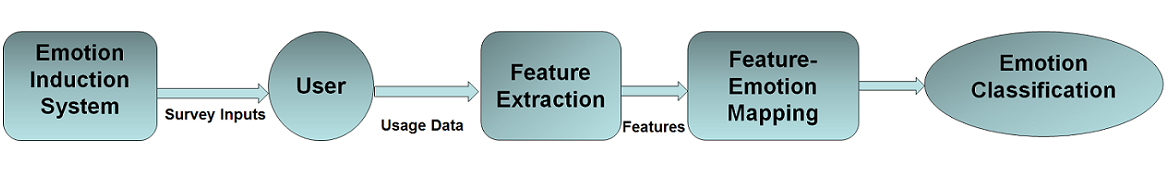
\includegraphics[width=5.25in,clip,keepaspectratio]{Chapters/figures/workingProcedure2.png}
\caption{Our proposed approach for emotion detection}
\label{Optional }
\end{figure}

